\documentclass[10pt,landscape]{article}
\usepackage[scaled=0.8]{helvet}

\usepackage{calc}
\usepackage{multicol}
\usepackage{ifthen}
\usepackage[a4paper,margin=3mm,landscape]{geometry}
\usepackage{amsmath,amsthm,amsfonts,amssymb}
\usepackage{hyperref}
\usepackage{newtxtext} 
\usepackage{enumitem}
\usepackage{amssymb}
\usepackage[table]{xcolor}
\usepackage{vwcol}
\usepackage{tikz}
\usepackage{wrapfig}
\usepackage{makecell}
% Testing %
\usepackage{blindtext}
\usetikzlibrary{calc}

\setlist{nosep}
\graphicspath{ {./images/} }

\pagestyle{empty}
\newenvironment{tightcenter}{%
  \setlength\topsep{0pt}
  \setlength\parskip{0pt}
  \begin{center}
}{%
  \end{center}
}

% redefine section commands to use less space
\makeatletter
\renewcommand{\section}{\@startsection{section}{1}{0mm}%
                                {-1ex plus -.5ex minus -.2ex}%
                                {0.5ex plus .2ex}%x
                                {\normalfont\large\bfseries}}
\renewcommand{\subsection}{\@startsection{subsection}{2}{0mm}%
                                {-1explus -.5ex minus -.2ex}%
                                {0.5ex plus .2ex}%
                                {\normalfont\normalsize\bfseries}}
\renewcommand{\subsubsection}{\@startsection{subsubsection}{3}{0mm}%
                                {-1ex plus -.5ex minus -.2ex}%
                                {1ex plus .2ex}%
                                {\normalfont\small\bfseries}}%
\renewcommand{\familydefault}{\sfdefault}
\renewcommand\rmdefault{\sfdefault}
% makes nested numbering (e.g. 1.1.1, 1.1.2, etc)
\renewcommand{\labelenumii}{\theenumii}
\renewcommand{\theenumii}{\theenumi.\arabic{enumii}.}
\renewcommand\labelitemii{•}
%  for logical not operator
\renewcommand{\lnot}{\mathord{\sim}}
\renewcommand{\bf}[1]{\textbf{#1}}
\newcommand{\abs}[1]{\vert #1 \vert}
\newcommand{\Mod}[1]{\ \mathrm{mod}\ #1}
\newcommand{\vv}[1]{\boldsymbol{#1}}
\newcommand{\VV}[1]{\overrightarrow{#1}}
\newcommand{\cvv}[1]{\left(\begin{smallmatrix}#1\end{smallmatrix}\right)}

\makeatother
\definecolor{myblue}{cmyk}{1,.72,0,.38}
% Define BibTeX command
\everymath\expandafter{\the\everymath \color{myblue}}
\def\BibTeX{{\rm B\kern-.05em{\sc i\kern-.025em b}\kern-.08em
    T\kern-.1667em\lower.7ex\hbox{E}\kern-.125emX}}
\let\iff\leftrightarrow
\let\Iff\Leftrightarrow
\let\then\rightarrow
\let\Then\Rightarrow

% Don't print section numbers
\setcounter{secnumdepth}{0}

\setlength{\parindent}{0pt}
\setlength{\parskip}{0pt plus 0.5ex}
%% this changes all items (enumerate and itemize)
\setlength{\leftmargini}{0.5cm}
\setlength{\leftmarginii}{0.5cm}
\setlist[itemize,1]{leftmargin=2mm,labelindent=1mm,labelsep=1mm}
\setlist[itemize,2]{leftmargin=4mm,labelindent=1mm,labelsep=1mm}

%My Environments
\newtheorem{example}[section]{Example}
% -----------------------------------------------------------------------

\begin{document}
\raggedright
\footnotesize
\begin{multicols*}{4}
  \setlength{\columnseprule}{0.25pt}
  \setlength{\premulticols}{1pt}
  \setlength{\postmulticols}{1pt}
  \setlength{\multicolsep}{1pt}
  \setlength{\columnsep}{2pt}

\section{Function and Limits}
\begin{itemize}
  \item $\lim\limits_{x\to \pm \infty}\frac{Ax^\alpha}{Bx^\beta} 
      \begin{cases} 
        0 & \text{if} \alpha < \beta\\
        \frac{A}{B} & \text{if} \alpha = \beta\\
        \pm \infty & \text{if} \alpha > \beta\\
      \end{cases}$
    \item $\lim\limits_{x\to c}\frac{sin(g(x))}{g(x)} = 1(\lim\limits_{x \to c}g(x) = 0)$
    \item $\lim\limits_{x\to c}\frac{tan(g(x))}{g(x)} = 1$
    \item $\lim\limits_{x\to 0}\frac{sin(x)}{x} = 1$
    \item $\lim\limits_{x\to 0}\frac{tan(x)}{x} = 1$
\end{itemize}


\section{Differentiation}
parametric differentiaton: $\frac{d^2y}{dx^2} = \frac{d}{dx}(\frac{dy}{dx}) = \frac{\frac{d}{dt}(\frac{dy}{dx})}{\frac{dx}{dt}}$

\begin{tabular}{|>{\color{black}}c | >{\color{black}}c|}
  \hline
  $f(x)$ & $f'(x)$
  \\ \hline
  \rule{0pt}{2.3ex}  % top spacing
  $\tan x$ & $\sec ^2 x$ \\
  $\csc x$ & $-\csc x \cot x$ \\
  $\sec x$ & $\sec x \tan x$ \\
  $\cot x$ & $- \csc ^2 x$
  \\ \hline
  \rule{0pt}{2.3ex}  % top spacing
  $a^{f(x)}$ & $\ln a \cdot f'(x)a^{f(x)}$ \\
  $\log_af(x)$ & $\log_a e \cdot \frac{f'(x)}{f(x)}$
  \\[1ex] \hline
  \rule{0pt}{3ex}  % top spacing
  $\sin^{-1} f(x)$ & $\frac{f'(x)}{\sqrt{1-[f(x)]^2}}, \ \ _{\vert f(x) \vert < 1}$ \\[1.5ex]
  $\cos^{-1} f(x)$ & $-\frac{f'(x)}{\sqrt{1-[f(x)]^2}}, \ \ _{\vert f(x) \vert < 1}$ \\[1.5ex]
  $\tan^{-1} f(x)$ & $\frac{f'(x)}{1 + [f(x)]^2}$ \\[1.5ex]
  $\cot^{-1} f(x)$ & $-\frac{f'(x)}{1 + [f(x)]^2}$ \\[1.5ex]
  $\sec^{-1} f(x)$ & $\frac{f'(x)}{\vert f(x) \vert \sqrt{[f(x)]^2-1}}$ \\[1.5ex]
  $\csc^{-1} f(x)$ & $-\frac{f'(x)}{\vert f(x) \vert \sqrt{[f(x)]^2-1}}$ \\[2ex]
  \hline
\end{tabular}

\textbf{Second Derivative} Test: $f'(c) = 0, f''(c) < 0$ then local max, $f''(c) > 0$ local min. 

\textbf{L'Hopital's Rule}: Given $\lim\limits_{x\to c}f(x) $ and $ g(x) = 0 / \pm \infty$ $ \lim\limits_{x \to c}\frac{f(x)}{g(x)} = \lim\limits_{x \to c}\frac{f'(x)}{g'(x)}$
\begin{itemize}
  \item Use for $\frac{0}{0}$ or $\frac{\infty}{\infty}$
\end{itemize}

\subsection*{Trigo Identities}
\begin{enumerate}
  \item $\sec^2x - 1 = \tan^2x$
  \item $\csc^2x - 1 = \cot^2x$
  \item $\sin A\cos A = \frac{1}{2}\sin2A$
  \item $\cos^2A = \frac{1}{2}(1+\cos2A)$
  \item $\sin^2A = \frac{1}{2}(1-\cos2A)$
  \item $\sin A\cos B = \frac{1}{2}(\sin(A + B) + \sin(A - B)$
  \item $\cos A\sin B = \frac{1}{2}(\sin(A + B) - \sin(A - B)$
  \item $\cos A\cos B = \frac{1}{2}(\cos(A + B) + \cos(A - B)$
  \item $\sin A\sin B = \frac{1}{2}(\cos(A + B) - \cos(A - B)$
\end{enumerate}

\section{Integration}

\begin{tabular}{|>{\color{black}}c | >{\color{black}}c|}
  \hline
  $f(x)$ & $\int f(x)$\\
  $\tan ax$ & $\frac{1}{a}\ln|\sec(ax)|$\\
  $\cot ax$ & $\frac{1}{a}\ln|\cot(ax)|$\\
  $\sec ax$ & $\frac{1}{a}\ln|\sec(ax) + tan(ax)|$\\
  $\csc ax$ & $\frac{1}{a}\ln|\csc(ax) + cot(ax)|$\\
  \hline
  $\frac{1}{a^2+(x+b)^2}$ & $\frac{1}{a}\tan^{-1}(\frac{x+b}{a})$\\
  $\frac{1}{\sqrt{a^2-(x+b)^2}}$ & $\sin^{-1}(\frac{x+b}{a})$\\
  $\frac{1}{a^2-(x+b)^2}$ & $\frac{1}{2a}\ln|\frac{x+b+a}{x+b-a}|$\\
  $\frac{1}{(x+b)^2-a^2}$ & $\frac{1}{2a}\ln|\frac{x+b-a}{x+b+a}|$\\
  \hline
\end{tabular}

\textbf{Substitution} $\int f(g(x)) \cdot g'(x) dx = \int f(u) du, u = g(x)$

\textbf{By Parts} $\int u v' dx = uv - \int u'v dx$, order: LIATE: Differentiate to integrate

\subsection{Application of Integration}
about x axis
\begin{itemize}
  \item Vol Disk:  $V = \pi \int^b_a f(x)^2 - g(x)^2 dx$
  \item Vol Shell: $V = 2\pi\int^b_a x|f(x)-g(x)|dx$ (absolute!!)
  \item Length of curve: $\int^b_a \sqrt{1+f'(x)^2}dx$
\end{itemize}
\section{Series}
TODO!!

\section{Vectors}
unit vector: $\hat{p} = \frac{p}{|p|}$, $\VV{AB} = \VV{OB} - \VV{OA}$
\begin{center}
    \begin{multicols}{2}
        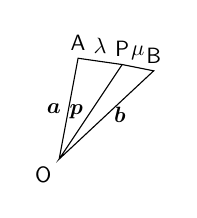
\begin{tikzpicture}[scale=0.8, every node/.style={transform shape}]
            \coordinate[label=below left:O] (O) at (0,0);
            \coordinate[label=A] (A) at (0.3,1.6);
            \coordinate[label=B] (B) at (1.5, 1.4);
            \coordinate[label=P] (P) at (1, 1.5);
            \draw (O) 
            -- node[left] {$\vv{a}$} (A) 
            -- node[above] {$\lambda$} (P)
            -- node[above] {$\mu$} (B) 
            -- node[right] {$\vv{b}$} (O) 
            -- node[left] {$\vv{p}$} (P);
        \end{tikzpicture}
        \\ \textbf{ratio theorem}
        \\* $\vv{p} = \frac{\mu\vv{a} + \lambda\vv{b}}{\lambda + \mu}$
        \newline
        \\ \textbf{midpoint theorem}
        \\* $\vv{p} = \frac{\vv{a} + \vv{b}}{2}$
    \end{multicols}
\end{center}
\subsection{Dot Product}
\begin{itemize}
  \item $\VV{a} \cdot \VV{b} = a_1b_1 + a_2b_2 + a_3b_3 = |a||b|\cos\theta$
  \item $a \perp b \Then a \cdot b = 0$
  \item $a \parallel b \Then a \cdot b = |a||b|$
\end{itemize}

\subsection{Cross Product}
$\vv{a} \times \vv{b} = \begin{vmatrix} 
\vv{i} & \vv{j} & \vv{k} \\ 
a_i & a_2 & a_3 \\
b_i & b_2 & b_3
\end{vmatrix} = \begin{pmatrix} (a_2b_3 - a_3b_2) \\ -(a_1b_3 - a_3b_1) \\ (a_1b_2 - a_2b_1) \end{pmatrix}$

\begin{center}
\begin{multicols}{2}
  $|\vv{a} \times \vv{b}| = |\vv{a}||\vv{b}|\sin\theta$
  $a \perp b \Then a \times b = |a||b|$
  $a \parallel b \Then a \times b = 0$
  Parallelogram = $|\vv{a} \times \vv{b}|$
\end{multicols}
\end{center}

\subsection{Projection}
\begin{multicols}{2}
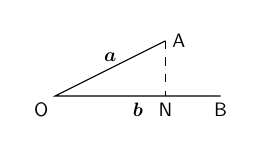
\begin{tikzpicture}[scale=0.7, every node/.style={transform shape}]
    \coordinate[label=below left:O] (O) at (0,0);
    \coordinate[label=right:A] (A) at (2, 1);
    \coordinate[label=below:B] (B) at (3, 0);
    \coordinate[label=below:N] (N) at (2, 0);
    \draw (A) 
        -- node[above] {$\vv{a}$} (O)
        -- node[below] {$\vv{b}$} (B); 
    \draw[shorten >=0pt, dashed] (A) -- (N);
\end{tikzpicture}
$\triangle ANO = \frac{1}{2} \abs{\VV{OA} \times \VV{ON}}$
\columnbreak

$\text{comp}_{\vv{b}}\vv{a} = |\vv{b}|\cos\theta = \frac{\vv{a}\cdot \vv{b}}{|\vv{a}|}$
$\text{proj}_{\vv{b}}\vv{a} = \text{comp}_{\vv{b}}\vv{a} \cdot \frac{a}{|a|} = \VV{ON} = \frac{\vv{a}\cdot \vv{b}}{\vv{a}\cdot \vv{a}}\vv{a} = \frac{\vv{a} \cdot \vv{b}}{|\vv{a}|^2}\vv{b}$
\end{multicols}

\subsection{Lines}
\begin{multicols}{2}
$\vv{r} = \vv{r}_0 + t\vv{v} = \langle x,y,z\rangle$ 
$\langle x_0,y_0,z_0\rangle + t\langle a,b,c\rangle$
$\begin{pmatrix}
  x_0 + at \\
  y_0 + bt \\
  z_0 + ct \\
\end{pmatrix}$
\end{multicols}
\subsection{Planes}
$\vv{n} = \langle a, b, c \rangle, \vv{r} = \langle x, y, z \rangle,\vv{r}_0\langle x_0, y_0, c_0 \rangle$\\
Scalar: $\vv{n} \cdot \vv{r} = \vv{n} \cdot \vv{r}_0$\\
Cartesian: $ax + by + cz = d$
\subsection{Distance from Point to Plane}
$\frac{|ax_0 + by_0 + cz_0 - d|}{\sqrt{a^2 + b^2 + c^2}}$

\section{Partial Derivatives}
\subsection{Chain Rule}
For $z(t) = f(x(t), y(t))$, 
\\* $\frac{dz}{dt} = \frac{\partial z}{\partial x}\frac{dx}{dt} + \frac{\partial z}{\partial y}\frac{dy}{dt}$

For $z(s, t) = f(x(s,t), y(s,t))$, 
\\* $\frac{\partial z}{\partial t} = \frac{\partial z}{\partial x}\frac{\partial x}{\partial t} + \frac{\partial z}{\partial y}\frac{\partial y}{\partial t}$
\\* $\frac{\partial z}{\partial s} = \frac{\partial z}{\partial x}\frac{\partial x}{\partial s} + \frac{\partial z}{\partial y}\frac{\partial y}{\partial s}$

Arc Length of $r(t)$: $\int^b_a |\vv{r}'(t)|dt$

\subsection{Implicit Differentiation}
$\frac{\partial z}{\partial x} =- \frac{F_x}{F_z}$
$\frac{\partial z}{\partial y} =- \frac{F_y}{F_z}$

\subsection{Directional Derivative}
Gradient vector at $f(x,y): \triangle f = f_x\vv{i} + f_y\vv{j}$

$D_uf(x, y) = \langle f_x, f_y \rangle \cdot \langle a, b \rangle = \langle f_x, f_y\rangle \cdot \hat{\vv{u}} = \triangle f \cdot \hat{\vv{u}}$ (Unit Vector)

Tangent Plane: $\triangle f \cdot \langle x-x_0, y-y_0,z-z_0\rangle = 0$

\subsection{Critical Points}
$D = f_{xx}(a,b)f_{yy}(a,b) - (f_{x,y}(a,b))^2$
\def\arraystretch{1.2}
\begin{tabular}{| c | c | c |}
  \hline $D$ & $f_{xx}(a,b)$ & \textbf{local}
  \\\hline + & + & \text{min}
  \\\hline + & - & \text{max}
  \\\hline - & \text{any} & \text{saddle point}
  \\\hline 0 & \text{any} & \text{no conclusion}
  \\\hline
\end{tabular} 
\section{Double Integrals}
\subsection{Type I}
\begin{multicols}{2}
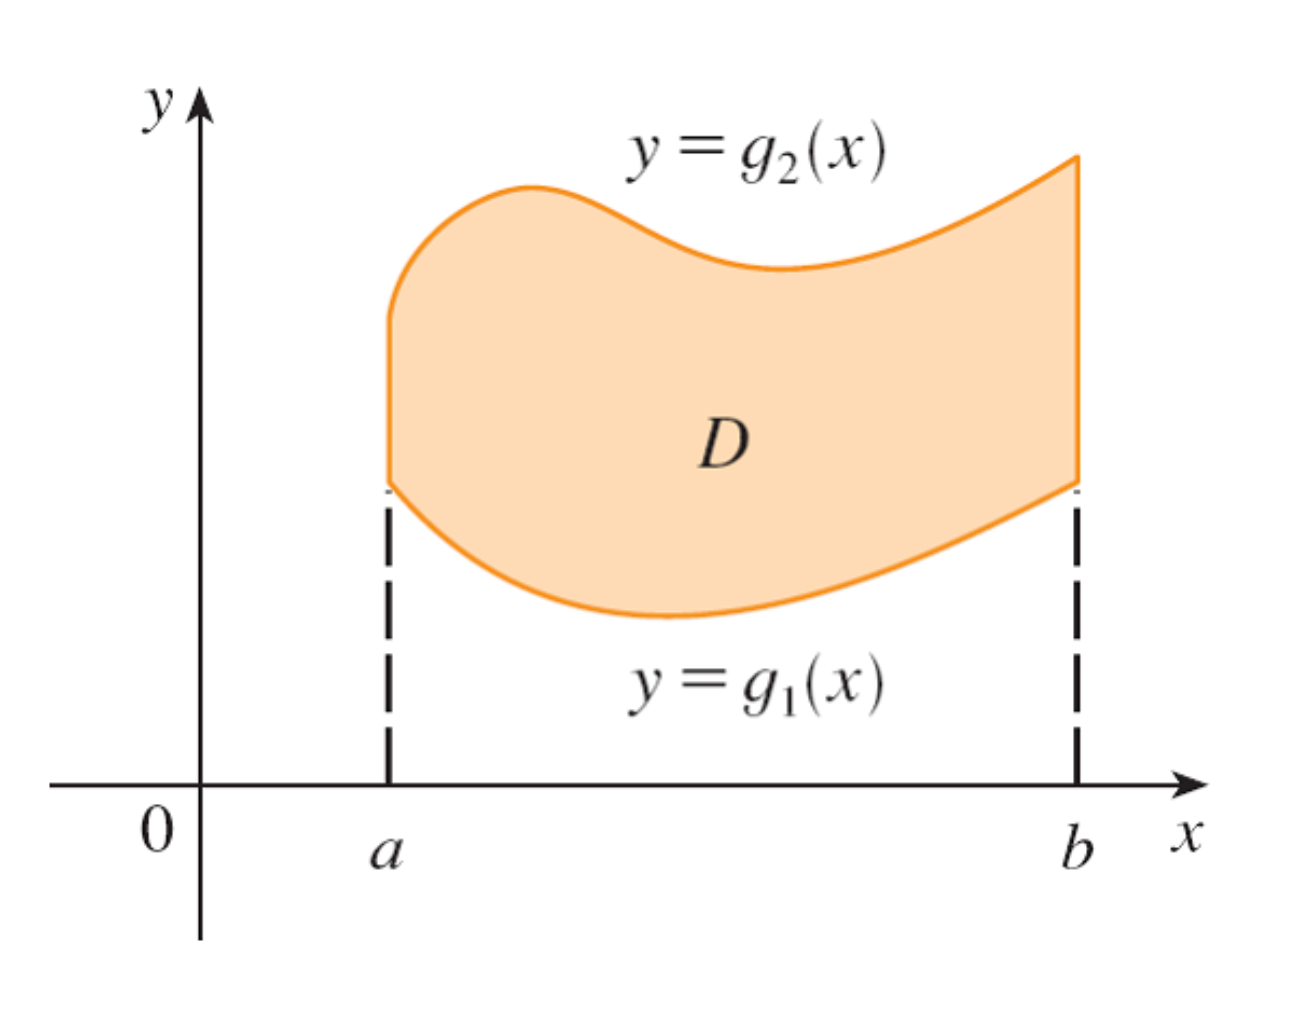
\includegraphics[width=\linewidth]{Type I}
\columnbreak

$\int^b_a\int^{g_2(x)}_{g_1(x)}f(x,y)dydx$
\newline
\newline
$D = \{(x,y): a \leq x \leq b,$ $g_1(x) \leq y \leq g_2(x)\}$
\end{multicols}
\subsection{Type II}
\begin{multicols}{2}
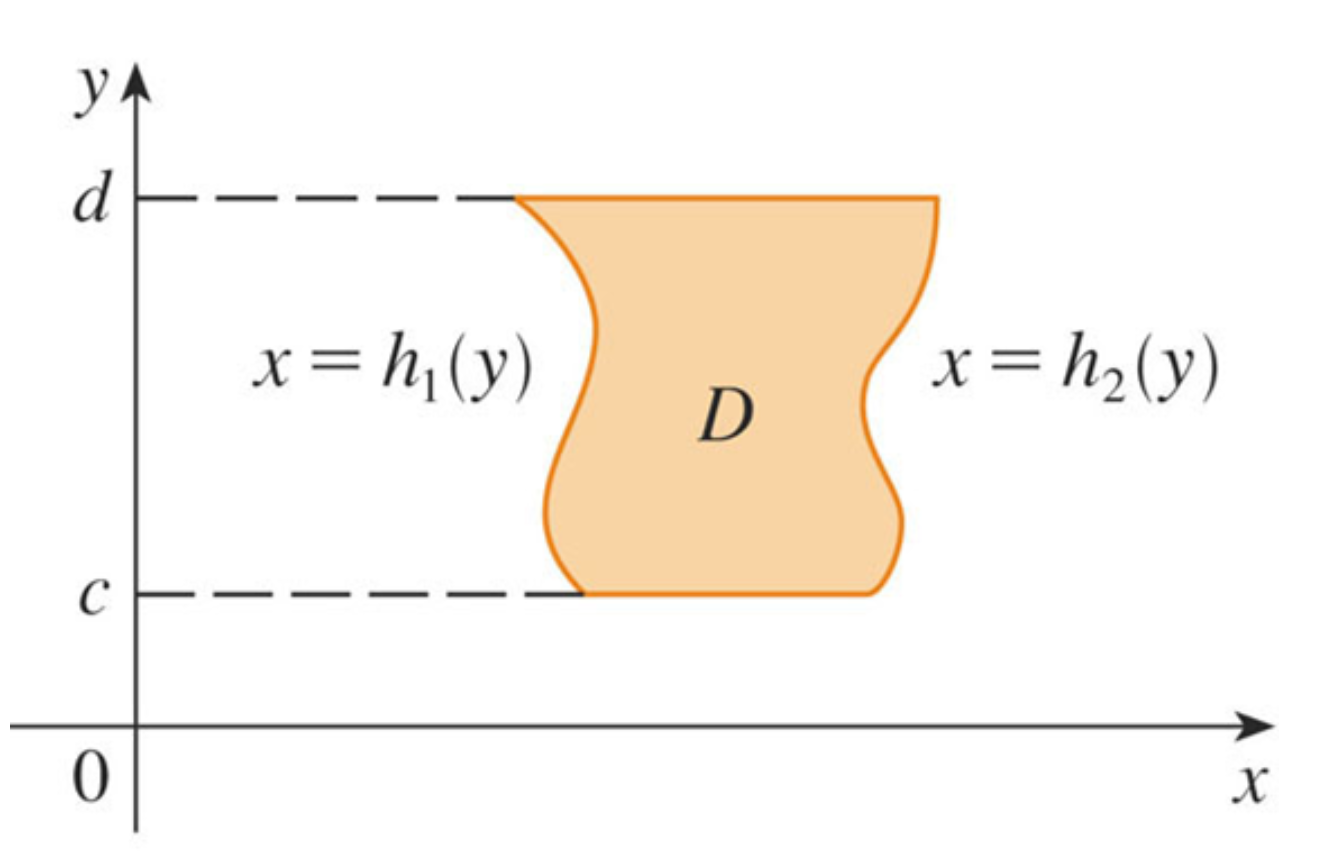
\includegraphics[width=\linewidth]{Type II}
\columnbreak

$\int^d_c\int^{h_2(y)}_{h_1(y)}f(x,y)dxdy$
\newline
\newline
$D = \{(x,y): c \leq y \leq d,$ $ h_1(y) \leq x \leq h_2(y)\}$
\end{multicols}

\subsection{Polar Coordinates}
\begin{multicols}{2}
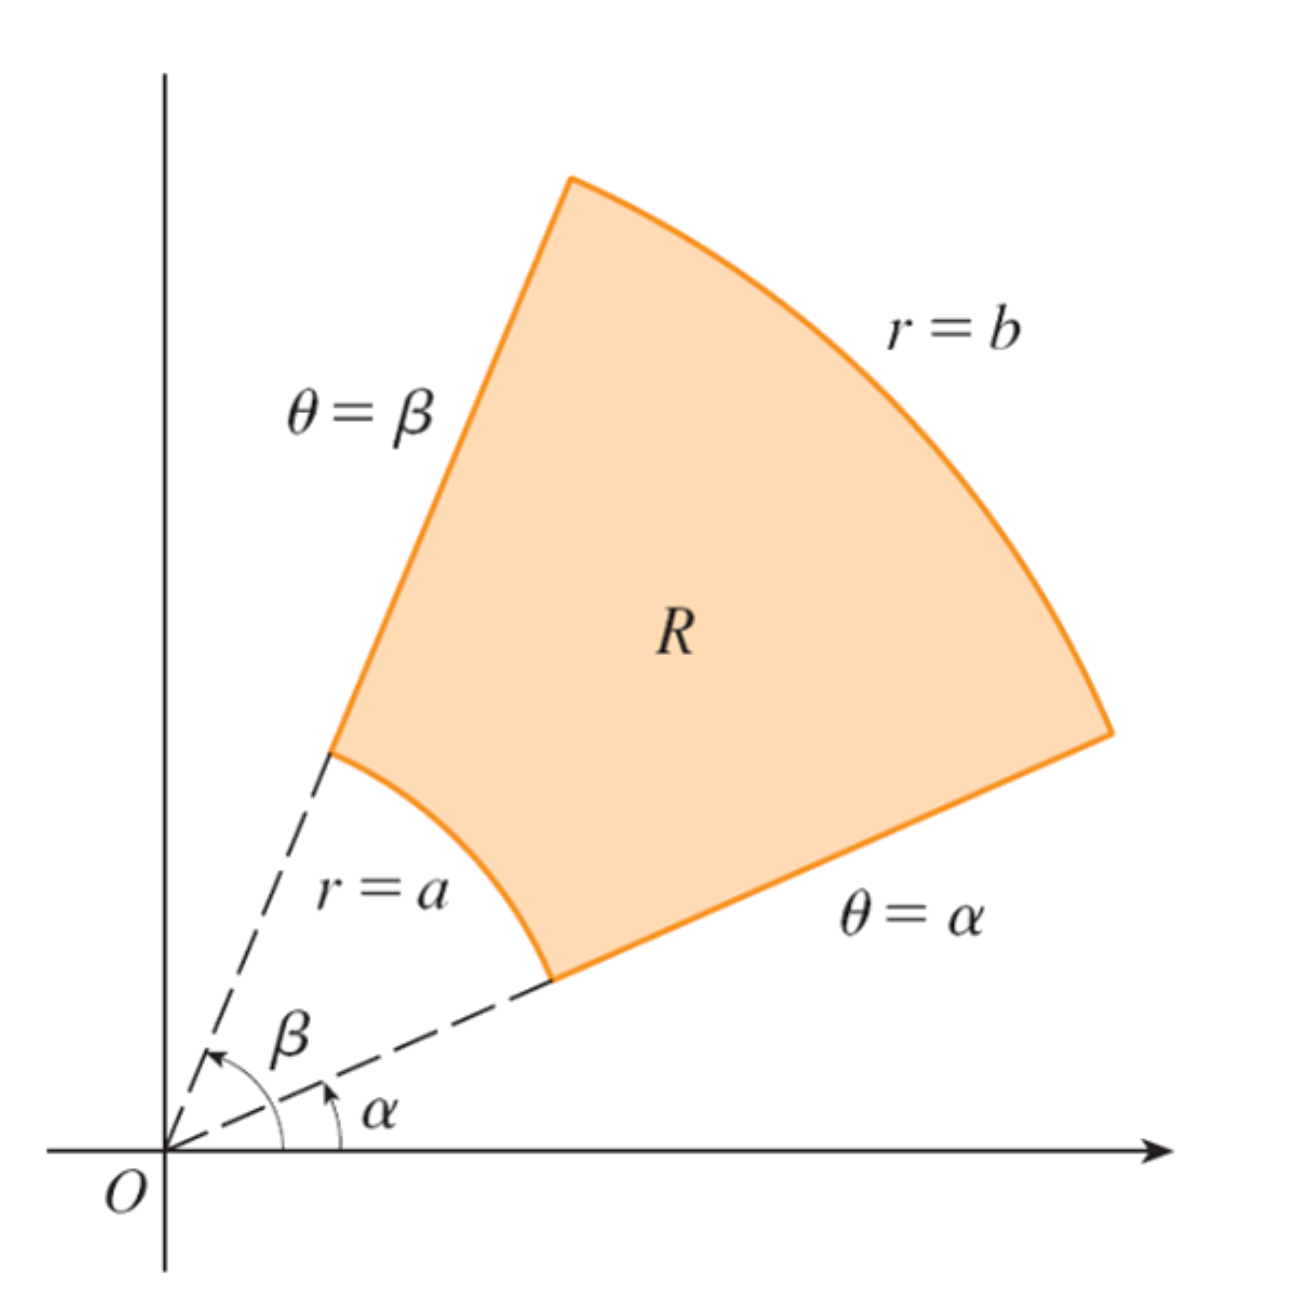
\includegraphics[width=\linewidth]{polar}
\columnbreak

$x = r\cos\theta$\\
$y = r\sin\theta$\\
$R = \{(r, \theta): 0 \leq a \leq r \leq b,$ $\alpha \leq \theta \leq \beta\}$
\newline
\newline
$\int^\beta_\alpha\int^b_af(r\cos\theta, r\sin\theta)rdrd\theta$
\end{multicols}

\subsection{Surface Area}
$S = \iint_R\sqrt{f_x^2 + f_y^2 + 1} dA$

\section{ODE}
\begin{tabular}{|>{\color{black}}c | >{\color{black}}c|}
  \hline
  form & change of variable \\
  \hline
  $\frac{dy}{dx} = f(x)g(y)$ & $\int \frac{1}{g(y)}dy = \int f(x)dx + C$\\
  \hline
  $y'=g(\frac{y}{x})$ & \makecell{Set $v = \frac{y}{x}$ \\ $\Then y' = v + xv' $}\\
  \hline
  \makecell{ $y'=f(ax + by + c)$\\ $\Then y' = \frac{ax+by+c}{\alpha x + \beta y + \gamma}$} & Set $v = ax+by$ \\
  \hline
  $y' + P(x)y = Q(x)$ & \makecell{$R = e^{\int P(x)dx}$ \\ $\Then y \cdot R = \int Q \cdot R dx $}\\
  $y' + P(x)y = Q(x)y^n$ & \makecell{$z = y^{1-n}$ \\ $\Then$ sub in Z \\ solve linear}\\
\end{tabular}

\section{Population Models}
\begin{center}
  $N_{\infty} = \frac{B}{s}$, $\hat{N} = $ Population Now
\begin{multicols}{2}
  \textbf{Malthus}\\
  $N(t) = \hat{N}e^{kt}$\\
  $k = B - D$

  \columnbreak
  \textbf{Logistic}\\
  $\frac{1}{N} = \frac{1}{N_{\infty}} + (\frac{1}{\hat{N}} - \frac{1}{N_{\infty}})e^{-Bt}$\\
  $N = \frac{N_{\infty}}{1+(\frac{N_{\infty}}{N} - 1)e^{-Bt}}$
\end{multicols}
\end{center}

\subsection{Uranium Decay into Thorium}
$U(t) = U_{0}e^{-k_ut}$, $k = \frac{\ln2}{\text{halflife}}, \frac{dU}{dt} = -k_{u}U$\\
Thorium: $T(t) = \frac{K_{u}U_{0}}{K_{t}-K_{u}}(e^{-k_{u}t} - e^{-k_{t}t}), \frac{dT}{dt} = k_{u}U - k_{T}T$


\end{multicols*}
\end{document}
